% ============================================================
% Question Bank: ch03-05 Multiplying Integers and Rational Numbers
% Topic Title: Multiplying Integers and Rational Numbers
% CCSS: 7.NS.A.2
% Questions: 27 (15 MC + 6 SA + 6 Graphical)
% ============================================================

% --- Multiple Choice Questions (15) ---

\begin{practiceQuestion}{3-5-q01}{mc}
\begin{questionText}
What is $(-6) \times 9$?
\end{questionText}
\choiceA{$54$}
\choiceB{$-54$}
\choiceC{$15$}
\choiceD{$-15$}
\correctAnswer{B}
\explanation{A negative times a positive is negative: $6 \times 9 = 54$, so $(-6) \times 9 = -54$.}
\end{practiceQuestion}

\begin{practiceQuestion}{3-5-q02}{mc}
\begin{questionText}
What is $(-4) \times (-7)$?
\end{questionText}
\choiceA{$-28$}
\choiceB{$28$}
\choiceC{$-11$}
\choiceD{$11$}
\correctAnswer{B}
\explanation{A negative times a negative is positive: $4 \times 7 = 28$, so $(-4) \times (-7) = 28$.}
\end{practiceQuestion}

\begin{practiceQuestion}{3-5-q03}{mc}
\begin{questionText}
What is $\left(-\dfrac{2}{3}\right) \times \dfrac{9}{4}$?
\end{questionText}
\choiceA{$\dfrac{3}{2}$}
\choiceB{$-\dfrac{3}{2}$}
\choiceC{$\dfrac{18}{12}$}
\choiceD{$-\dfrac{18}{12}$}
\correctAnswer{B}
\explanation{Multiply: $\dfrac{2 \times 9}{3 \times 4} = \dfrac{18}{12} = \dfrac{3}{2}$. Negative × positive = negative: $-\dfrac{3}{2}$.}
\end{practiceQuestion}

\begin{practiceQuestion}{3-5-q04}{mc}
\begin{questionText}
A stock loses $\$3$ per share each day for $5$ days. What is the total change in value per share?
\end{questionText}
\choiceA{$\$15$}
\choiceB{$-\$15$}
\choiceC{$\$8$}
\choiceD{$-\$8$}
\correctAnswer{B}
\explanation{$(-3) \times 5 = -15$. Each day the stock drops $\$3$, so over $5$ days it drops $\$15$.}
\end{practiceQuestion}

\begin{practiceQuestion}{3-5-q05}{mc}
\begin{questionText}
What is $(-5) \times (-2) \times (-3)$?
\end{questionText}
\choiceA{$30$}
\choiceB{$-30$}
\choiceC{$10$}
\choiceD{$-10$}
\correctAnswer{B}
\explanation{Odd number of negatives gives a negative: $5 \times 2 \times 3 = 30$, so the result is $-30$.}
\end{practiceQuestion}

\begin{practiceQuestion}{3-5-q06}{mc}
\begin{questionText}
Which expression has a positive product?
\end{questionText}
\choiceA{$(-3) \times 2 \times (-1) \times (-4)$}
\choiceB{$(-3) \times (-2) \times 1 \times (-4)$}
\choiceC{$(-3) \times (-2) \times (-1) \times (-4)$}
\choiceD{$3 \times (-2) \times 1 \times 4$}
\correctAnswer{C}
\explanation{Count the negatives. A: $3$ negatives → negative. B: $3$ negatives → negative. C: $4$ negatives (even) → positive. D: $1$ negative → negative.}
\end{practiceQuestion}

\begin{practiceQuestion}{3-5-q07}{mc}
\begin{questionText}
What is $(-1.5) \times 4$?
\end{questionText}
\choiceA{$6.0$}
\choiceB{$-6.0$}
\choiceC{$5.5$}
\choiceD{$-5.5$}
\correctAnswer{B}
\explanation{$1.5 \times 4 = 6.0$. Negative times positive is negative: $-6.0$.}
\end{practiceQuestion}

\begin{practiceQuestion}{3-5-q08}{mc}
\begin{questionText}
What is $\left(-\dfrac{3}{5}\right) \times \left(-\dfrac{5}{3}\right)$?
\end{questionText}
\choiceA{$-1$}
\choiceB{$1$}
\choiceC{$-\dfrac{9}{25}$}
\choiceD{$\dfrac{9}{25}$}
\correctAnswer{B}
\explanation{These are reciprocals: $\dfrac{3 \times 5}{5 \times 3} = \dfrac{15}{15} = 1$. Two negatives make a positive: $1$.}
\end{practiceQuestion}

\begin{practiceQuestion}{3-5-q09}{mc}
\begin{questionText}
What is $(-8) \times 0$?
\end{questionText}
\choiceA{$-8$}
\choiceB{$8$}
\choiceC{$0$}
\choiceD{undefined}
\correctAnswer{C}
\explanation{Any number multiplied by $0$ is $0$: $(-8) \times 0 = 0$.}
\end{practiceQuestion}

\begin{practiceQuestion}{3-5-q10}{mc}
\begin{questionText}
A scuba diver descends at $2.5$ meters per minute. What is the diver's position after $6$ minutes?
\end{questionText}
\choiceA{$-15$ meters}
\choiceB{$15$ meters}
\choiceC{$-8.5$ meters}
\choiceD{$8.5$ meters}
\correctAnswer{A}
\explanation{$(-2.5) \times 6 = -15$ meters. Descending is negative, so multiply the rate by time.}
\end{practiceQuestion}

\begin{practiceQuestion}{3-5-q11}{mc}
\begin{questionText}
What is $\dfrac{7}{8} \times \left(-\dfrac{4}{7}\right)$?
\end{questionText}
\choiceA{$-\dfrac{1}{2}$}
\choiceB{$\dfrac{1}{2}$}
\choiceC{$-\dfrac{28}{56}$}
\choiceD{$\dfrac{11}{15}$}
\correctAnswer{A}
\explanation{$\dfrac{7 \times 4}{8 \times 7} = \dfrac{28}{56} = \dfrac{1}{2}$. Positive × negative = negative: $-\dfrac{1}{2}$.}
\end{practiceQuestion}

\begin{practiceQuestion}{3-5-q12}{mc}
\begin{questionText}
Which statement about multiplying integers is always true?
\end{questionText}
\choiceA{The product of two negative integers is negative}
\choiceB{The product of a positive and a negative integer is positive}
\choiceC{The product of two positive integers is negative}
\choiceD{The product of two negative integers is positive}
\correctAnswer{D}
\explanation{Negative × negative = positive. This is always true by the sign rules for multiplication.}
\end{practiceQuestion}

\begin{practiceQuestion}{3-5-q13}{mc}
\begin{questionText}
What is $(-3)^3$?
\end{questionText}
\choiceA{$9$}
\choiceB{$-9$}
\choiceC{$27$}
\choiceD{$-27$}
\correctAnswer{D}
\explanation{$(-3)^3 = (-3) \times (-3) \times (-3) = 9 \times (-3) = -27$. An odd exponent keeps the negative sign.}
\end{practiceQuestion}

\begin{practiceQuestion}{3-5-q14}{mc}
\begin{questionText}
What is $(-0.4) \times (-0.3)$?
\end{questionText}
\choiceA{$-0.12$}
\choiceB{$0.12$}
\choiceC{$-0.7$}
\choiceD{$0.7$}
\correctAnswer{B}
\explanation{$0.4 \times 0.3 = 0.12$. Negative × negative = positive: $0.12$.}
\end{practiceQuestion}

\begin{practiceQuestion}{3-5-q15}{mc}
\begin{questionText}
A company's revenue changes by $-\$1{,}200$ each month for $4$ months. What is the total change?
\end{questionText}
\choiceA{$\$4{,}800$}
\choiceB{$-\$4{,}800$}
\choiceC{$-\$1{,}204$}
\choiceD{$\$3{,}600$}
\correctAnswer{B}
\explanation{$(-1{,}200) \times 4 = -4{,}800$. The revenue decreases a total of $\$4{,}800$.}
\end{practiceQuestion}

% --- Short Answer Questions (6) ---

\begin{practiceQuestion}{3-5-q16}{sa}
\begin{questionText}
What is $(-12) \times (-5)$?
\end{questionText}
\correctAnswer{$60$}
\explanation{Negative × negative = positive: $12 \times 5 = 60$.}
\end{practiceQuestion}

\begin{practiceQuestion}{3-5-q17}{sa}
\begin{questionText}
What is $\left(-\dfrac{3}{4}\right) \times \dfrac{2}{5}$?
\end{questionText}
\correctAnswer{$-\dfrac{6}{20}$ or $-\dfrac{3}{10}$}
\explanation{$\dfrac{3 \times 2}{4 \times 5} = \dfrac{6}{20} = \dfrac{3}{10}$. Negative × positive = negative: $-\dfrac{3}{10}$.}
\end{practiceQuestion}

\begin{practiceQuestion}{3-5-q18}{sa}
\begin{questionText}
The temperature drops $3°$F every hour for $7$ hours. What is the total change?
\end{questionText}
\correctAnswer{$-21°$F}
\explanation{$(-3) \times 7 = -21°$F. Each hour drops $3°$, so $7$ hours drops $21°$.}
\end{practiceQuestion}

\begin{practiceQuestion}{3-5-q19}{sa}
\begin{questionText}
What is $(-2) \times (-3) \times (-4) \times 1$?
\end{questionText}
\correctAnswer{$-24$}
\explanation{$3$ negative factors (odd) → negative. $2 \times 3 \times 4 \times 1 = 24$. Result: $-24$.}
\end{practiceQuestion}

\begin{practiceQuestion}{3-5-q20}{sa}
\begin{questionText}
What is $(-1.2) \times (-3.5)$?
\end{questionText}
\correctAnswer{$4.2$}
\explanation{$1.2 \times 3.5 = 4.2$. Two negatives: positive. Result is $4.2$.}
\end{practiceQuestion}

\begin{practiceQuestion}{3-5-q21}{sa}
\begin{questionText}
What is $\left(-\dfrac{1}{2}\right)^4$?
\end{questionText}
\correctAnswer{$\dfrac{1}{16}$}
\explanation{$\left(-\dfrac{1}{2}\right)^4 = \dfrac{1}{16}$. Even exponent ($4$) makes the result positive.}
\end{practiceQuestion}

% --- Graphical Questions (3 GMC + 3 GSA) ---

\begin{practiceQuestion}{3-5-q22}{gmc}
\begin{questionText}
The number line below models a multiplication. What multiplication is shown?

\begin{center}
\begin{tikzpicture}
  \draw[thick,->] (-16.5,0) -- (1.5,0);
  \foreach \x in {-15,-12,-9,-6,-3,0} \draw (\x/1,0.1) -- (\x/1,-0.1) node[below,font=\small] {$\x$};
  \draw[thick,->,funRed] (0,0.35) -- (-5,0.35);
  \node[above,font=\small] at (-2.5,0.4) {$-5$};
  \draw[thick,->,funRed] (-5,0.35) -- (-10,0.35);
  \node[above,font=\small] at (-7.5,0.4) {$-5$};
  \draw[thick,->,funRed] (-10,0.35) -- (-15,0.35);
  \node[above,font=\small] at (-12.5,0.4) {$-5$};
\end{tikzpicture}
\end{center}
\end{questionText}
\choiceA{$3 \times 5 = 15$}
\choiceB{$3 \times (-5) = -15$}
\choiceC{$(-3) \times 5 = -15$}
\choiceD{$(-3) \times (-5) = 15$}
\correctAnswer{B}
\explanation{Three jumps of $-5$ each: $3 \times (-5) = -15$. Starting at $0$ and landing at $-15$.}
\end{practiceQuestion}

\begin{practiceQuestion}{3-5-q23}{gmc}
\begin{questionText}
The table shows patterns. What is the next value?

\begin{center}
\begin{tabular}{|c|c|}
\hline
\textbf{Factor} & \textbf{Product with $-4$} \\
\hline
$3$ & $-12$ \\ \hline
$2$ & $-8$ \\ \hline
$1$ & $-4$ \\ \hline
$0$ & $0$ \\ \hline
$-1$ & ? \\ \hline
\end{tabular}
\end{center}
\end{questionText}
\choiceA{$-4$}
\choiceB{$-8$}
\choiceC{$4$}
\choiceD{$8$}
\correctAnswer{C}
\explanation{Pattern: each product increases by $4$: $-12, -8, -4, 0, \ldots$ Next: $0 + 4 = 4$. Also: $(-1) \times (-4) = 4$.}
\end{practiceQuestion}

\begin{practiceQuestion}{3-5-q24}{gmc}
\begin{questionText}
A parking garage charges $\$2.50$ per floor descended below ground. The diagram shows $4$ underground floors. What is the total charge to reach floor B4?

\begin{center}
\begin{tikzpicture}[scale=0.6]
  \draw[thick] (-2,0) -- (2,0) node[right,font=\small] {Ground: $0$};
  \draw[thick] (-2,-1.5) -- (2,-1.5) node[right,font=\small] {B1: $-1$};
  \draw[thick] (-2,-3) -- (2,-3) node[right,font=\small] {B2: $-2$};
  \draw[thick] (-2,-4.5) -- (2,-4.5) node[right,font=\small] {B3: $-3$};
  \draw[thick] (-2,-6) -- (2,-6) node[right,font=\small] {B4: $-4$};
  \draw[thick,<-,funRed] (-1.5,0) -- (-1.5,-6);
  \node[left,font=\small] at (-1.5,-3) {$4$ floors};
\end{tikzpicture}
\end{center}
\end{questionText}
\choiceA{$\$2.50$}
\choiceB{$\$5.00$}
\choiceC{$\$7.50$}
\choiceD{$\$10.00$}
\correctAnswer{D}
\explanation{$4$ floors $\times$ $\$2.50$ per floor $= \$10.00$. Multiply the rate by the number of floors.}
\end{practiceQuestion}

\begin{practiceQuestion}{3-5-q25}{gsa}
\begin{questionText}
Use the integer chips model below to find the product $(-3) \times 2$.

\begin{center}
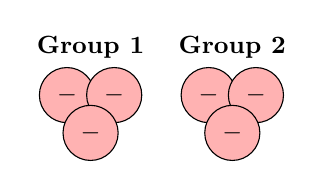
\begin{tikzpicture}[scale=0.6]
  \node[font=\small] at (0,2) {\textbf{Group 1}};
  \node[circle,draw,fill=red!30,minimum size=0.7cm,font=\small] at (-0.5,1) {$-$};
  \node[circle,draw,fill=red!30,minimum size=0.7cm,font=\small] at (0.5,1) {$-$};
  \node[circle,draw,fill=red!30,minimum size=0.7cm,font=\small] at (0,0.2) {$-$};
  \node[font=\small] at (3,2) {\textbf{Group 2}};
  \node[circle,draw,fill=red!30,minimum size=0.7cm,font=\small] at (2.5,1) {$-$};
  \node[circle,draw,fill=red!30,minimum size=0.7cm,font=\small] at (3.5,1) {$-$};
  \node[circle,draw,fill=red!30,minimum size=0.7cm,font=\small] at (3,0.2) {$-$};
\end{tikzpicture}
\end{center}
\end{questionText}
\correctAnswer{$-6$}
\explanation{Two groups of $3$ negative chips: $2 \times (-3) = -6$. Count all negative chips: $6$ negatives $= -6$.}
\end{practiceQuestion}

\begin{practiceQuestion}{3-5-q26}{gsa}
\begin{questionText}
The table shows a pattern. Complete the last row.

\begin{center}
\begin{tabular}{|c|c|c|}
\hline
$a$ & $b$ & $a \times b$ \\
\hline
$-2$ & $5$ & $-10$ \\ \hline
$-2$ & $3$ & $-6$ \\ \hline
$-2$ & $1$ & $-2$ \\ \hline
$-2$ & $-1$ & $2$ \\ \hline
$-2$ & $-3$ & ? \\ \hline
\end{tabular}
\end{center}
\end{questionText}
\correctAnswer{$6$}
\explanation{$(-2) \times (-3) = 6$. Also, the pattern shows products increasing by $4$: $-10, -6, -2, 2, 6$.}
\end{practiceQuestion}

\begin{practiceQuestion}{3-5-q27}{gsa}
\begin{questionText}
The bar graph shows the daily profit ($+$) or loss ($-$) for a lemonade stand. If the pattern repeats $3$ times, what is the total earnings?

\begin{center}
\begin{tikzpicture}[scale=0.6]
  \draw[thick,->] (0,-2.5) -- (0,5);
  \draw[thick,->] (0,0) -- (4.5,0);
  \foreach \y in {-2,-1,1,2,3,4} \draw (-0.15,\y) -- (0.15,\y) node[left=3pt,font=\footnotesize] {\y};
  \fill[funGreen] (0.5,0) rectangle (1.2,4);
  \fill[funRed] (1.8,0) rectangle (2.5,-2);
  \node[below,font=\footnotesize] at (0.85,-0.3) {Day 1};
  \node[below,font=\footnotesize] at (2.15,-0.3) {Day 2};
  \node[right,font=\footnotesize] at (0,4.5) {\$};
\end{tikzpicture}
\end{center}
\end{questionText}
\correctAnswer{$\$6$}
\explanation{One cycle: $4 + (-2) = 2$. Three cycles: $2 \times 3 = \$6$.}
\end{practiceQuestion}
